\begin{figure}[!htb]
\begin{center}
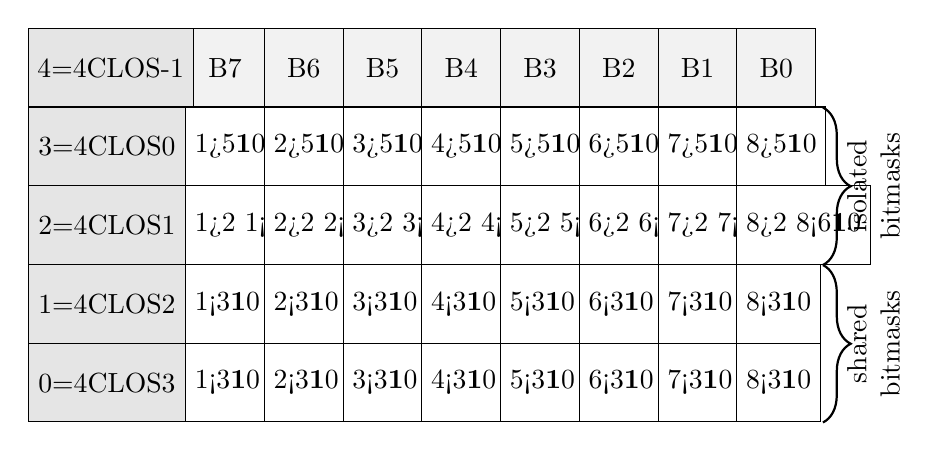
\begin{tikzpicture}

	\foreach \x [evaluate = \bindex using int(8-\x)] in {1,...,8}
		    	\node at (\x,4)[rectangle, draw=black, fill=black!5, minimum height = 1cm, minimum width = 1cm, anchor=south west] (r1\x) 
							{B\bindex};

	\foreach \x in {1,...,8}
		    	\node at (\x,3)[rectangle, draw=black, fill=white, minimum height = 1cm, minimum width = 1cm, anchor=south west] (r2\x) 
							{\ifthenelse{\x>5}{\textbf{1}}{0}};

	\foreach \x in {1,...,8}
		    	\node at (\x,2)[rectangle, draw=black, fill=white, minimum height = 1cm, minimum width = 1cm, anchor=south west] (r3\x) 
							{\ifthenelse{\x>2 \AND \x<6}{\textbf{1}}{0}};

	\foreach \x in {1,...,8}
		    	\node at (\x,1)[rectangle, draw=black, fill=white, minimum height = 1cm, minimum width = 1cm, anchor=south west] (r4\x) 
							{\ifthenelse{\x<3}{\textbf{1}}{0}};


	\foreach \x in {1,...,8}
		    	\node at (\x,0)[rectangle, draw=black, fill=white, minimum height = 1cm, minimum width = 1cm, anchor=south west] (r5\x) 
							{\ifthenelse{\x<3}{\textbf{1}}{0}};


	\foreach \y [evaluate = \closindex using int(3-\y)] in {4,...,0}
		    	\node at (-1,\y)[rectangle, draw=black, fill=black!10, minimum height = 1cm, minimum width = 2cm, anchor=south west] (r6\y) 
							{\ifthenelse{\y=4}{CLOS}{\closindex}};

	\draw[thick, decorate, decoration={brace,mirror,amplitude=10pt}] (9.1,2) -- (9.1,4) node [below, align=center, midway, rotate=90, text width=2cm] {\\isolated bitmasks};
	\draw[thick, decorate, decoration={brace,mirror,amplitude=10pt}] (9.1,0) -- (9.1,2) node [below, align=center, midway, rotate=90, text width=2cm] {\\shared bitmasks};

	%\node (isolatedmasks) at (11, 3) [text width=3cm, align=right]{Isolated Bitmasks};
	%\node (sharedmasks) at (11, 1) [text width=3cm, align=right]{Shared Bitmasks};	

	%\begin{scope}[>=latex]
	%\draw [thick, ->] (r28) to [bend left=45] (isolatedmasks.center);
	%\draw [thick, ->] (r38) to [bend left=45] (isolatedmasks.center);
	%\end{scope}

\end{tikzpicture}
\end{center}
\ifreport
\caption{Example of LLC Partitioning via Bitmasks. Three cache partitions are created by the bitmask registers. 
		First two are isolated ($3/8$ of LLC each) from the rest and the third is shared ($1/4$ of LLC).}
\fi
\label{fig-cat-bitmasks}
\end{figure}
